\documentclass{article}
\usepackage{array}
\usepackage{graphicx}

\usepackage[latin1]{inputenc}
\usepackage{tikz}
\usetikzlibrary{calc, shapes, arrows, positioning}

\newcommand{\prog}[1]{{\tt\em #1}}

\tikzstyle{bamfile} = [rectangle, draw, fill=yellow!20, text width=2cm, text centered, node distance=1.5cm, rounded corners, minimum height=0.34cm]
\tikzstyle{ssjfile} = [bamfile, fill=red!40]
\tikzstyle{sscfile} = [bamfile, fill=blue!40]
\tikzstyle{external} = [rectangle, draw, fill=green!20, text width=1.5cm, text centered, rounded corners]
\tikzstyle{line} = [draw, -latex']

\begin{document}
\thispagestyle{empty}
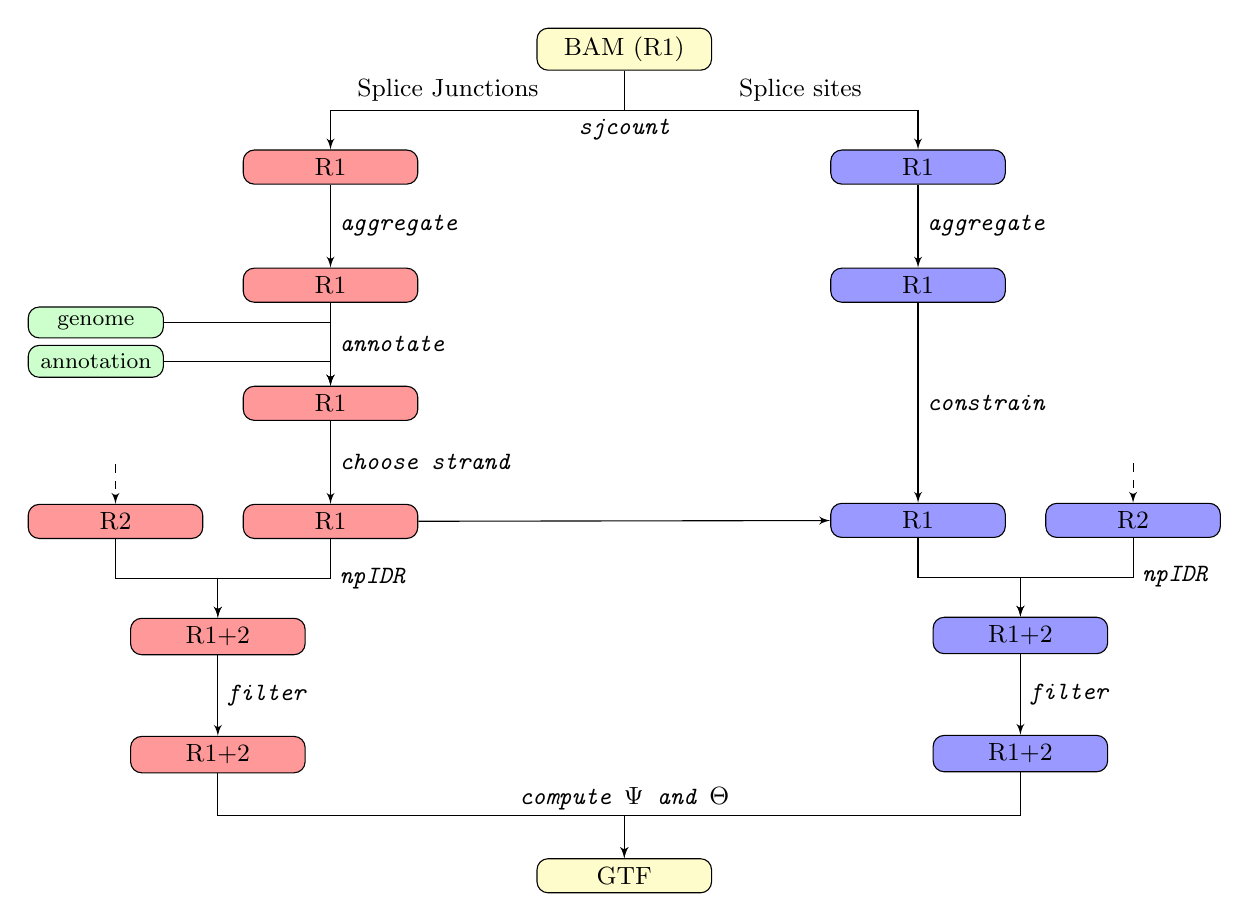
\begin{tikzpicture}
\small
\node [bamfile] (bam) {BAM (R1)};
\node [ssjfile, below left  = 1cm  and 1.5cm of bam] (ssj6) {R1};
\node [sscfile, below right = 1cm  and 1.5cm of bam] (ssc6) {R1};
\node [ssjfile, below of = ssj6] (ssj6+3) {R1};
\node [sscfile, below of = ssc6] (ssc6+3) {R1};
\node [ssjfile, below of = ssj6+3] (ssj6+3+2) {R1};
\node [ssjfile, below of = ssj6+3+2] (ssj6+3+2s) {R1};
\node [external, above left = 0.6cm and 1cm of ssj6+3+2] (genome) {\footnotesize genome};
\node [external, above left = 0.1cm and 1cm of ssj6+3+2] (annot) {\footnotesize annotation};
\path[line] (genome.east) -| (ssj6+3+2.north);
\path[line] (annot.east) -| (ssj6+3+2.north);
\node [sscfile, below = 2.54cm of ssc6+3] (ssc6+3s) {R1};
\path[line] let \p1=(bam.south), \p2=(ssj6.north) in (bam.south) --  +(0,0.5*\y2-0.5*\y1) node[below] {\prog{sjcount}} -| node [pos=0.3, above] {Splice Junctions} (ssj6.north);
\path[line] let \p1=(bam.south), \p2=(ssc6.north) in (bam.south) --  +(0,0.5*\y2-0.5*\y1)  -| node [pos=0.3, above] {Splice sites} (ssc6.north);
\path[line] (ssj6) -- node [right] {\prog{aggregate}} (ssj6+3);
\path[line] (ssj6+3) -- node [right] {\prog{annotate}} (ssj6+3+2);
\path[line] (ssj6+3+2) -- node [right] {\prog{choose strand}} (ssj6+3+2s);
\path[line] (ssc6) -- node [right] {\prog{aggregate}} (ssc6+3);
\path[line] (ssj6+3+2s) --  (ssc6+3s);
\path[line] (ssc6+3)  -- node[right] {\prog{constrain}} (ssc6+3s);
\node [ssjfile, left = 0.5cm of ssj6+3+2s] (ssj6+3+2sr2) {R2};
\node [sscfile, right = 0.5cm of ssc6+3s] (ssc6+3sr2) {R2};
\path[line,dashed] (ssj6+3+2sr2.north) ++(0,0.5cm) -- (ssj6+3+2sr2.north);
\path[line,dashed] (ssc6+3sr2.north) ++(0,0.5cm) -- (ssc6+3sr2.north);
\node [ssjfile, below left = 1cm and -0.8cm of ssj6+3+2s] (ssj12) {R1+2};
\path[line] let \p1=(ssj6+3+2sr2.south), \p2=(ssj12.north) in (ssj6+3+2sr2.south) --  +(0,0.5*\y2-0.5*\y1) -| (ssj12.north);
\path[line] let \p1=(ssj6+3+2s.south), \p2=(ssj12.north) in (ssj6+3+2s.south) -- node[below right] {\prog{npIDR}}  +(0,0.5*\y2-0.5*\y1) -| (ssj12.north);
\node [sscfile, below left = 1cm and -0.8cm of ssc6+3sr2] (ssc12) {R1+2};
\path[line] let \p1=(ssc6+3sr2.south), \p2=(ssc12.north) in (ssc6+3sr2.south) --  node[below right] {\prog{npIDR}} +(0,0.5*\y2-0.5*\y1) -| (ssc12.north);
\path[line] let \p1=(ssc6+3s.south), \p2=(ssc12.north) in (ssc6+3s.south) -- +(0,0.5*\y2-0.5*\y1) -| (ssc12.north);
\node [ssjfile, below of = ssj12] (ssj12f) {R1+2};
\node [sscfile, below of = ssc12] (ssc12f) {R1+2};
\path[line] (ssj12) -- node[right] {\prog{filter}} (ssj12f);
\path[line] (ssc12) -- node[right] {\prog{filter}} (ssc12f);
\node [bamfile, below = 10cm of bam] (gtf) {GTF};
\path[line] let \p1=(ssj12f.south), \p2=(gtf.north) in (ssj12f.south) --  +(0,0.5*\y2-0.5*\y1) -| (gtf.north);
\path[line] let \p1=(ssc12f.south), \p2=(gtf.north) in (ssc12f.south) --  +(0,0.5*\y2-0.5*\y1) -| (gtf.north) node[above=0.5cm] {\prog{compute $\Psi$ and $\Theta$}};
\end{tikzpicture}
\end{document}

